\documentclass[12pt]{article}

\usepackage{graphicx}
\usepackage{listings}
\usepackage{hyperref}
\usepackage{float}

\graphicspath{ {./images/} }

\oddsidemargin 0mm
\evensidemargin 0mm
\textwidth 160mm
\textheight 200mm

\pagestyle {plain}
\pagenumbering{arabic}

\newcounter{stepnum}

\title{CS/SE 2XC3 Lab 2 Report}
\author{
  Glotov, Oleg\\ L03, 400174037\\
  \texttt{glotovo@mcmaster.ca}
  \and
  Willson, Emma\\ L02, 400309856\\
  \texttt{willsone@mcmaster.ca}
  }
\date{\today}

\begin{document}

\maketitle

This report includes the main observations that we found in this week's lab, along with the analysis of our results.

\newpage 
\section{Timing Data}
In this section, we analyze the test results of three functions and give our best judgement of how each of these functions is growing in $n$.
\subsection{\(f(n)\)}
For the data set of $f(n)$, the trend line appears to be linear. From the chart below we can see that the $R^2$ is 0.9992 for the linear equation. It is already a very good result.

\begin{figure}[h!]
\centering
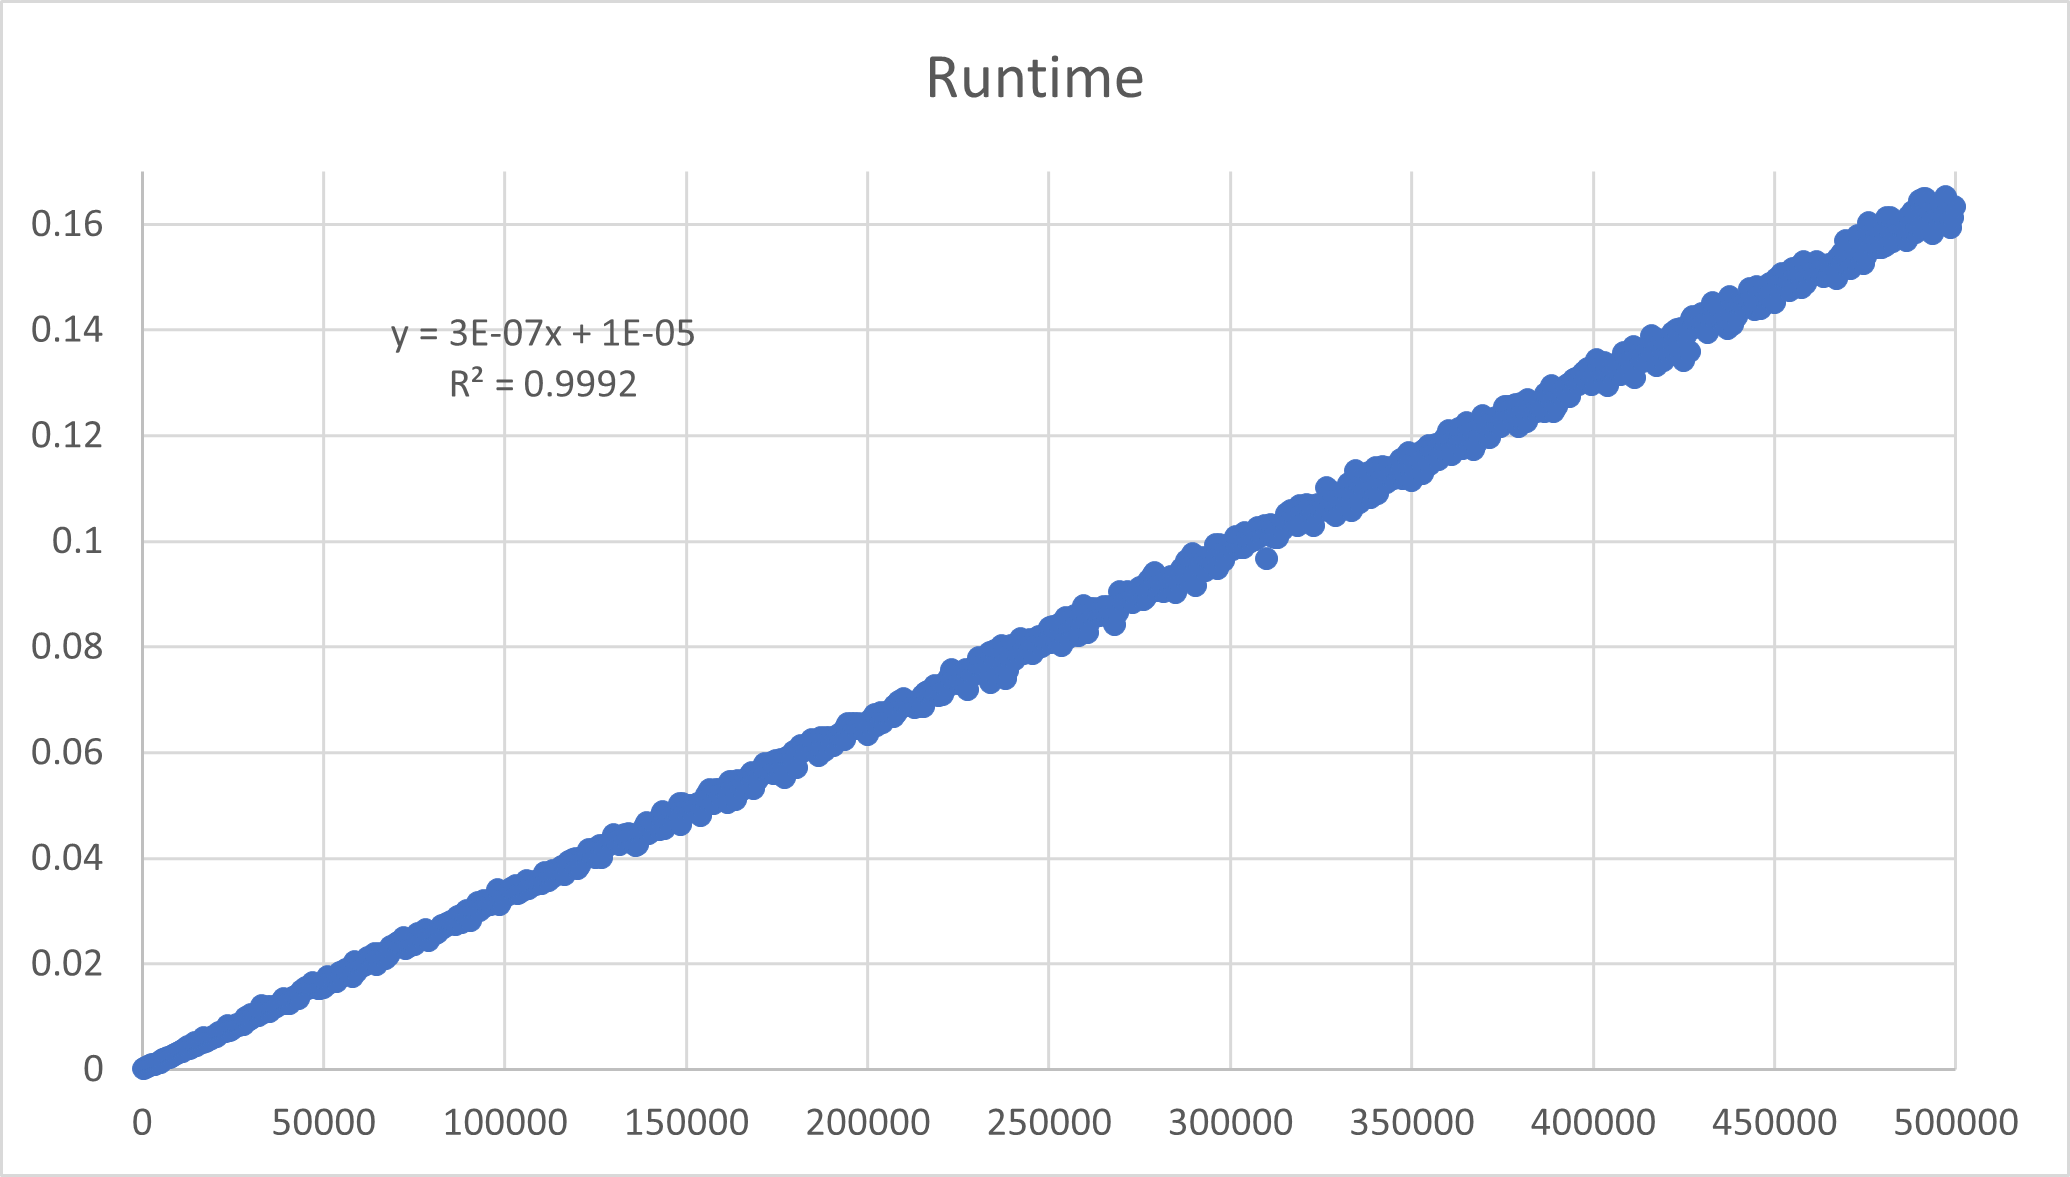
\includegraphics[width=0.6\textwidth,height=\textheight,keepaspectratio]{fn_Tn}
\caption{linear fitting for $f(n)$}
\label{Figure: fn_1}
\end{figure}
\noindent Therefore, we can conclude that $f(n) = O(n)$. 

\subsection{\(g(n)\)}
When we graph the data set for $g(n)$, the trend line appears to be polynomial. From the chart below we can see that the $R^2$ is 0.9883 for the quadratic equation. 

\begin{figure}[H]
\centering
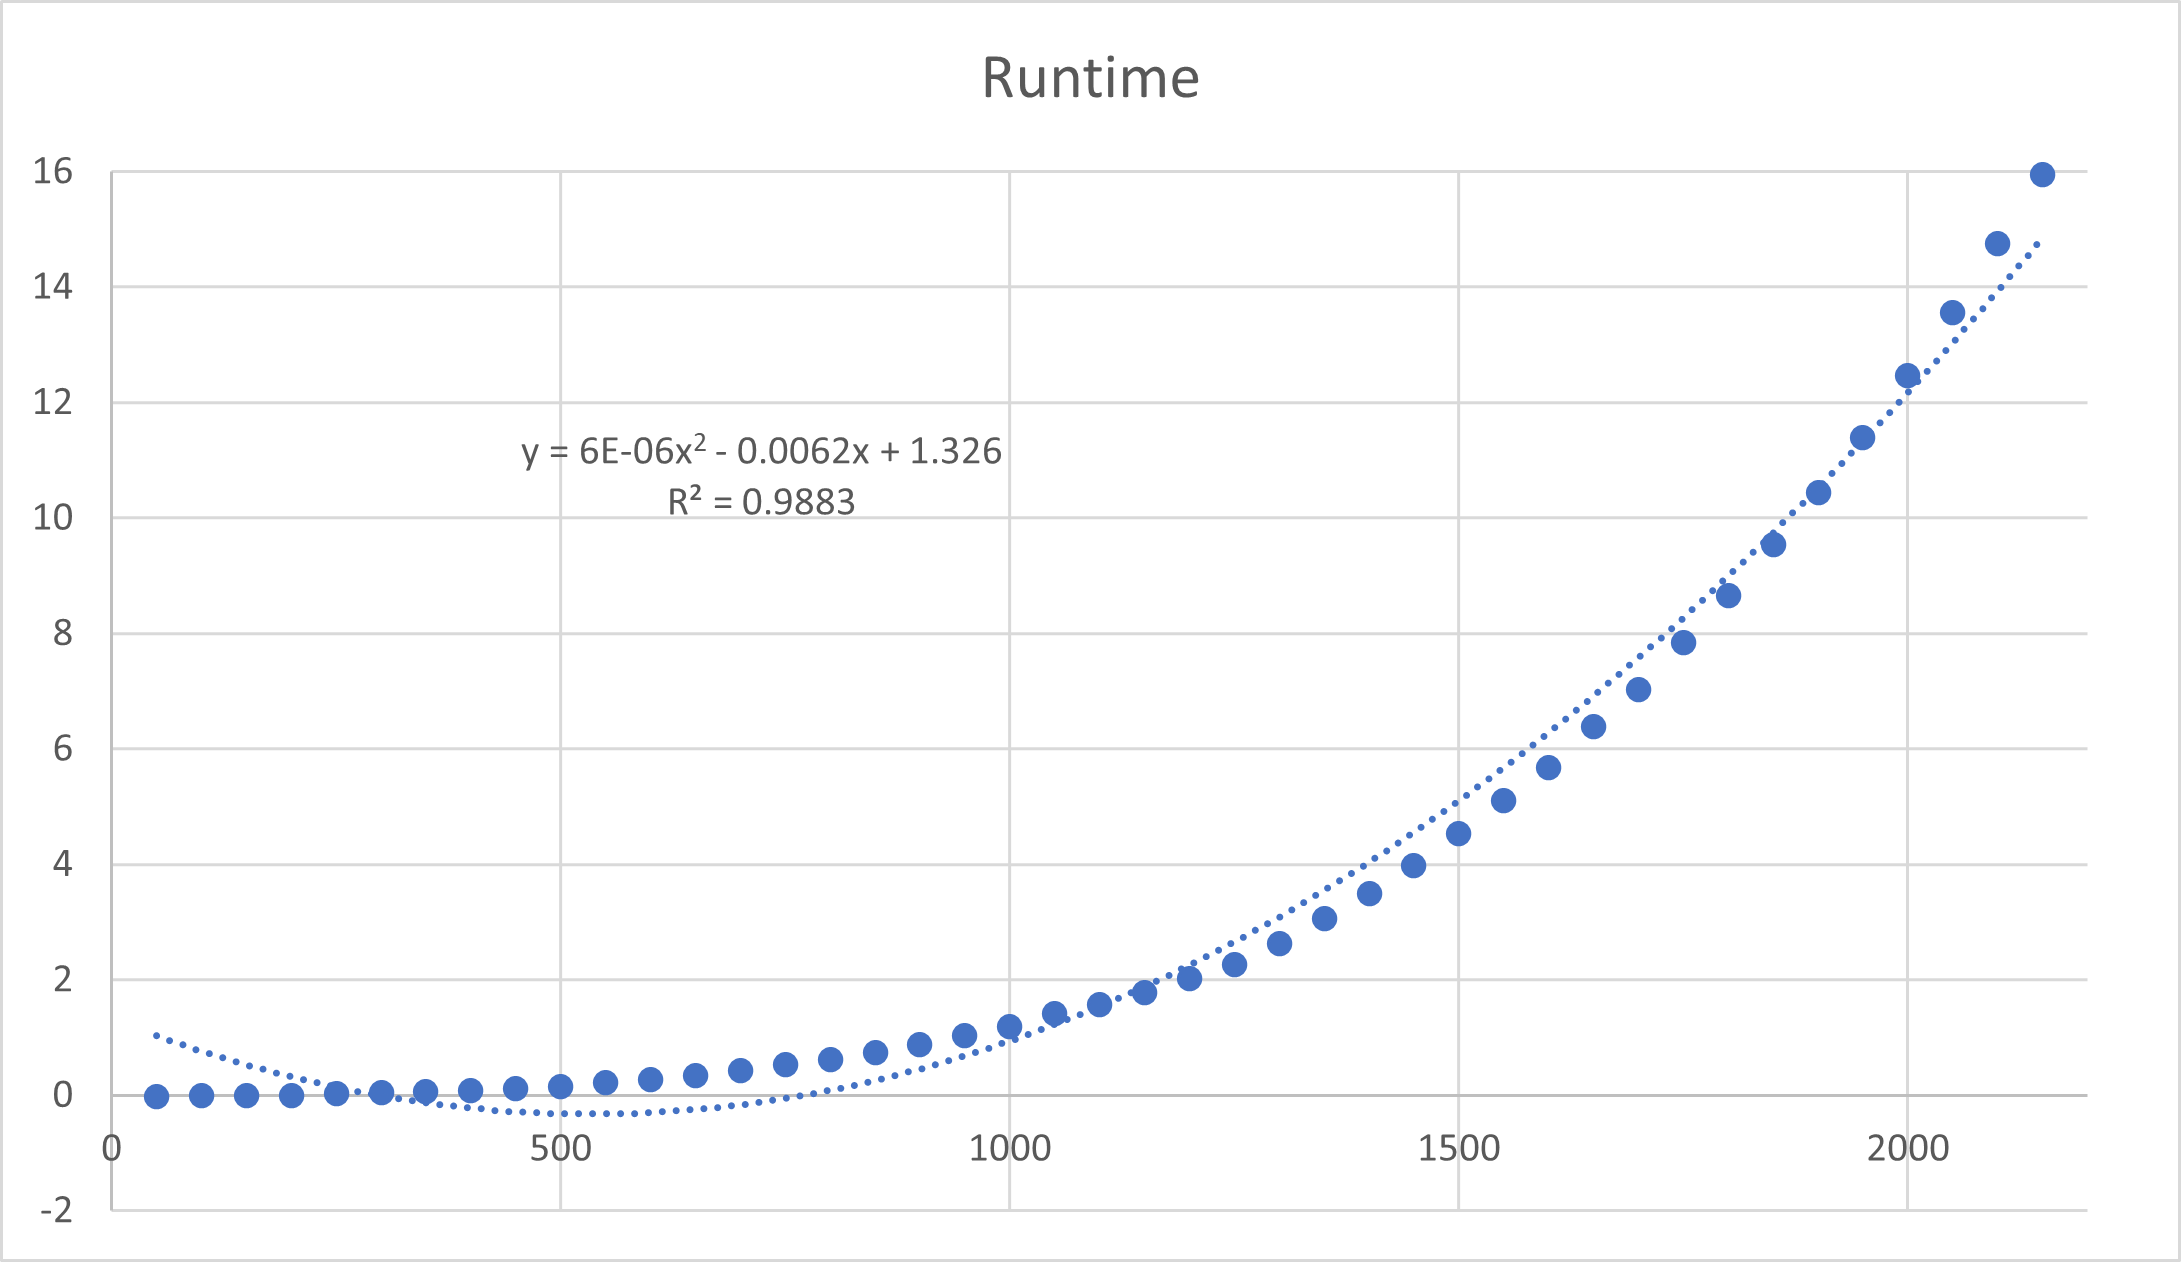
\includegraphics[width=0.6\textwidth,height=\textheight,keepaspectratio]{gn_Tn}
\caption{polynomial fitting for $g(n)$}
\label{Figure: gn_1}
\end{figure}

\noindent We will try to improve the $R^2$ by finding the value of $k$ in $T(n) = cn^k$. We do so by taking the logarithm of both sides of this equation: $\log{T}=\log{c}+k\log{n}$ and plotting $\log{T}$ against $\log{n}$. 

\begin{figure}[H]
\centering
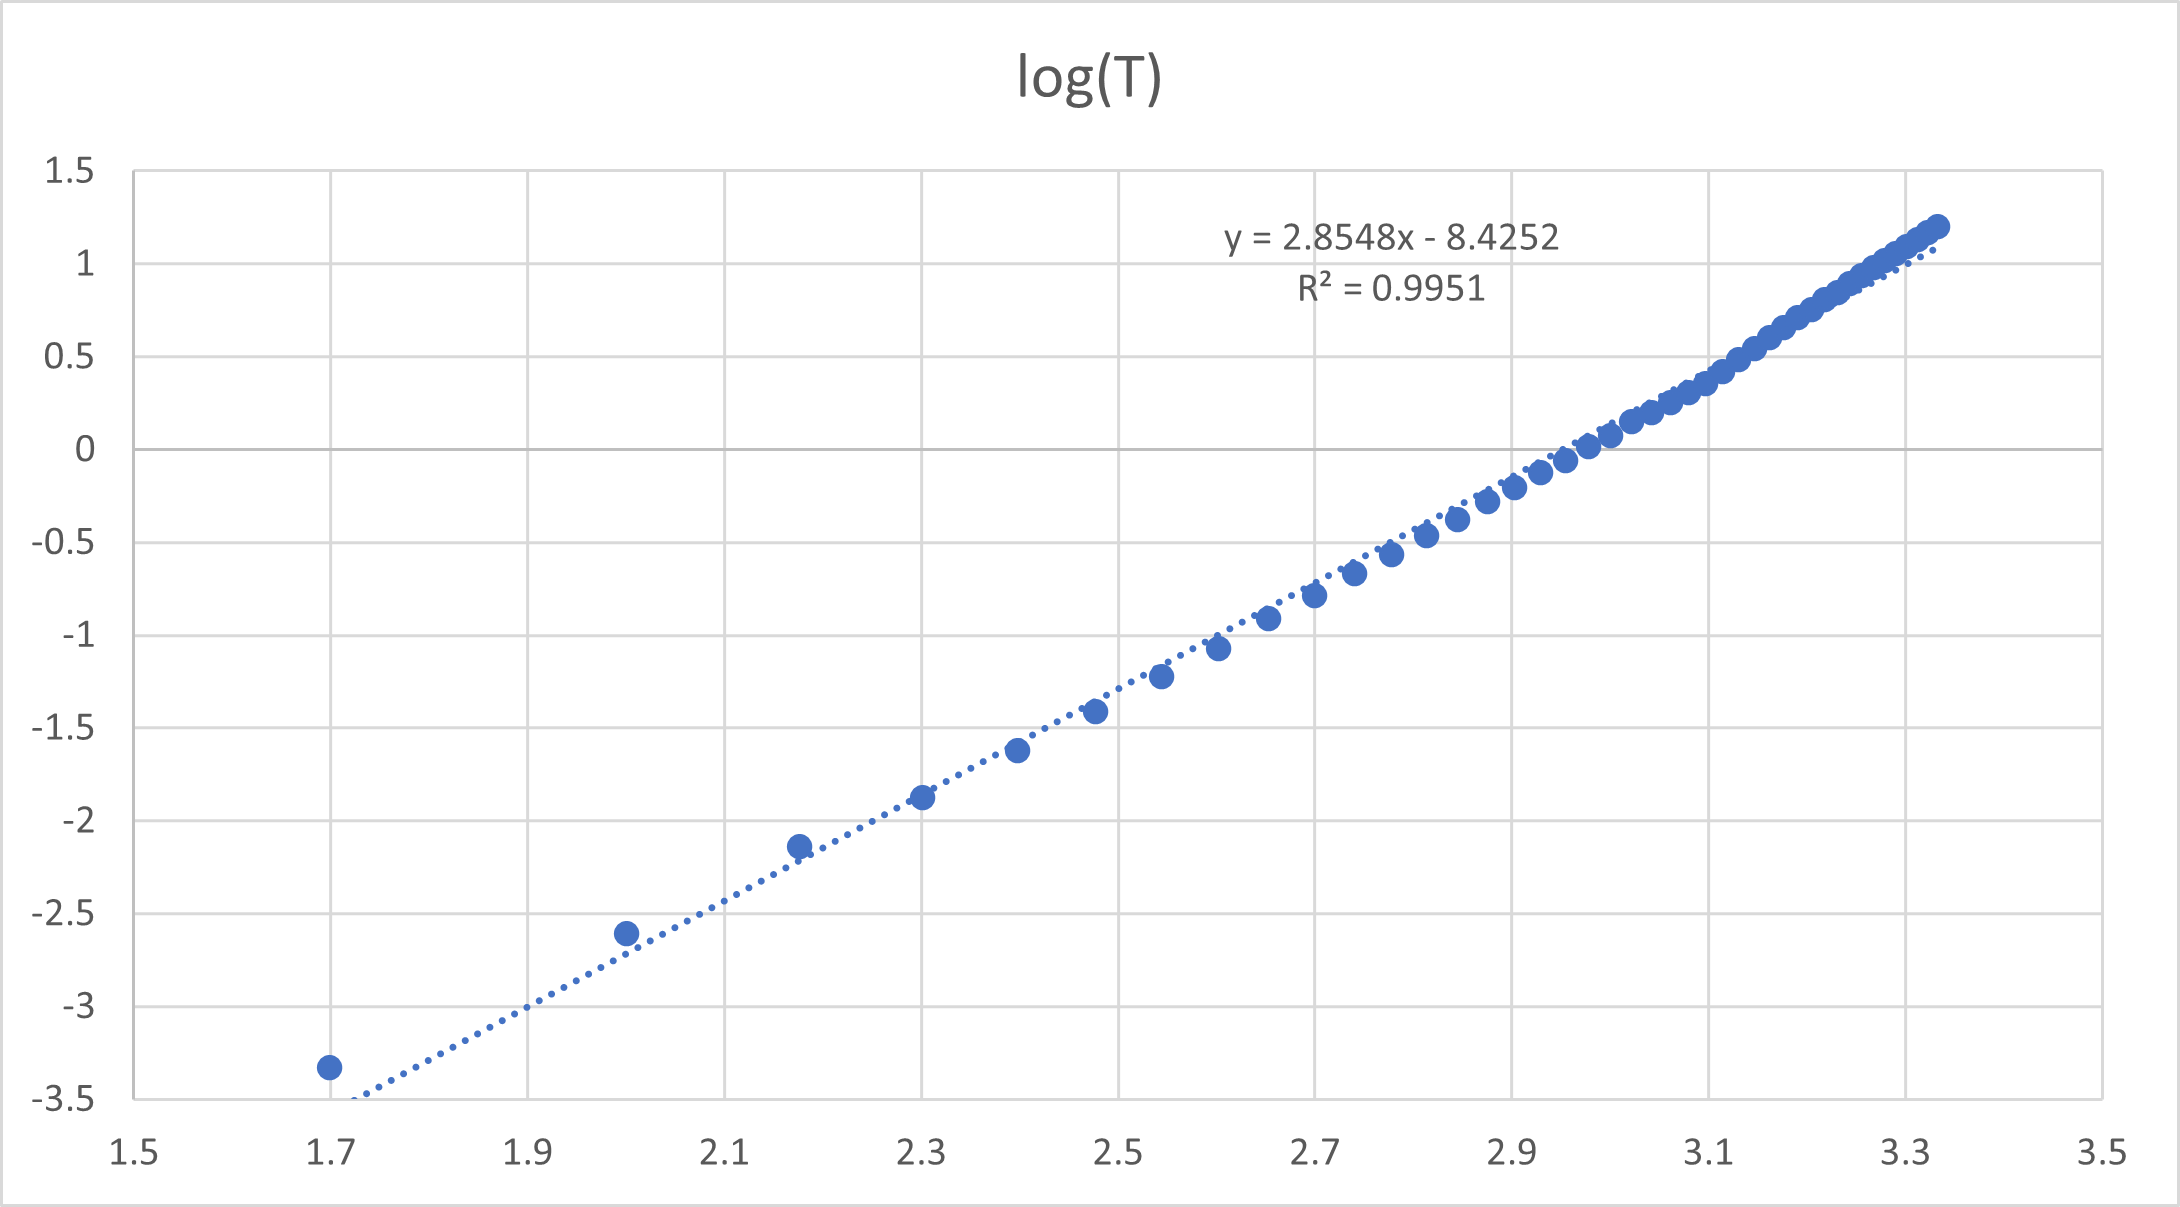
\includegraphics[width=0.6\textwidth,height=\textheight,keepaspectratio]{gn_logT}
\caption{polynomial fitting for $\log{T}$}
\label{Figure: gn_2}
\end{figure}

\noindent When we choose a linear trend line for this relation, we see that $k$, the slope, is 2.8548, which is closer to 3. When we recalculate the polynomial trend line for the original data with $k=3$, we see that this is a better fit.

\begin{figure}[H]
\centering
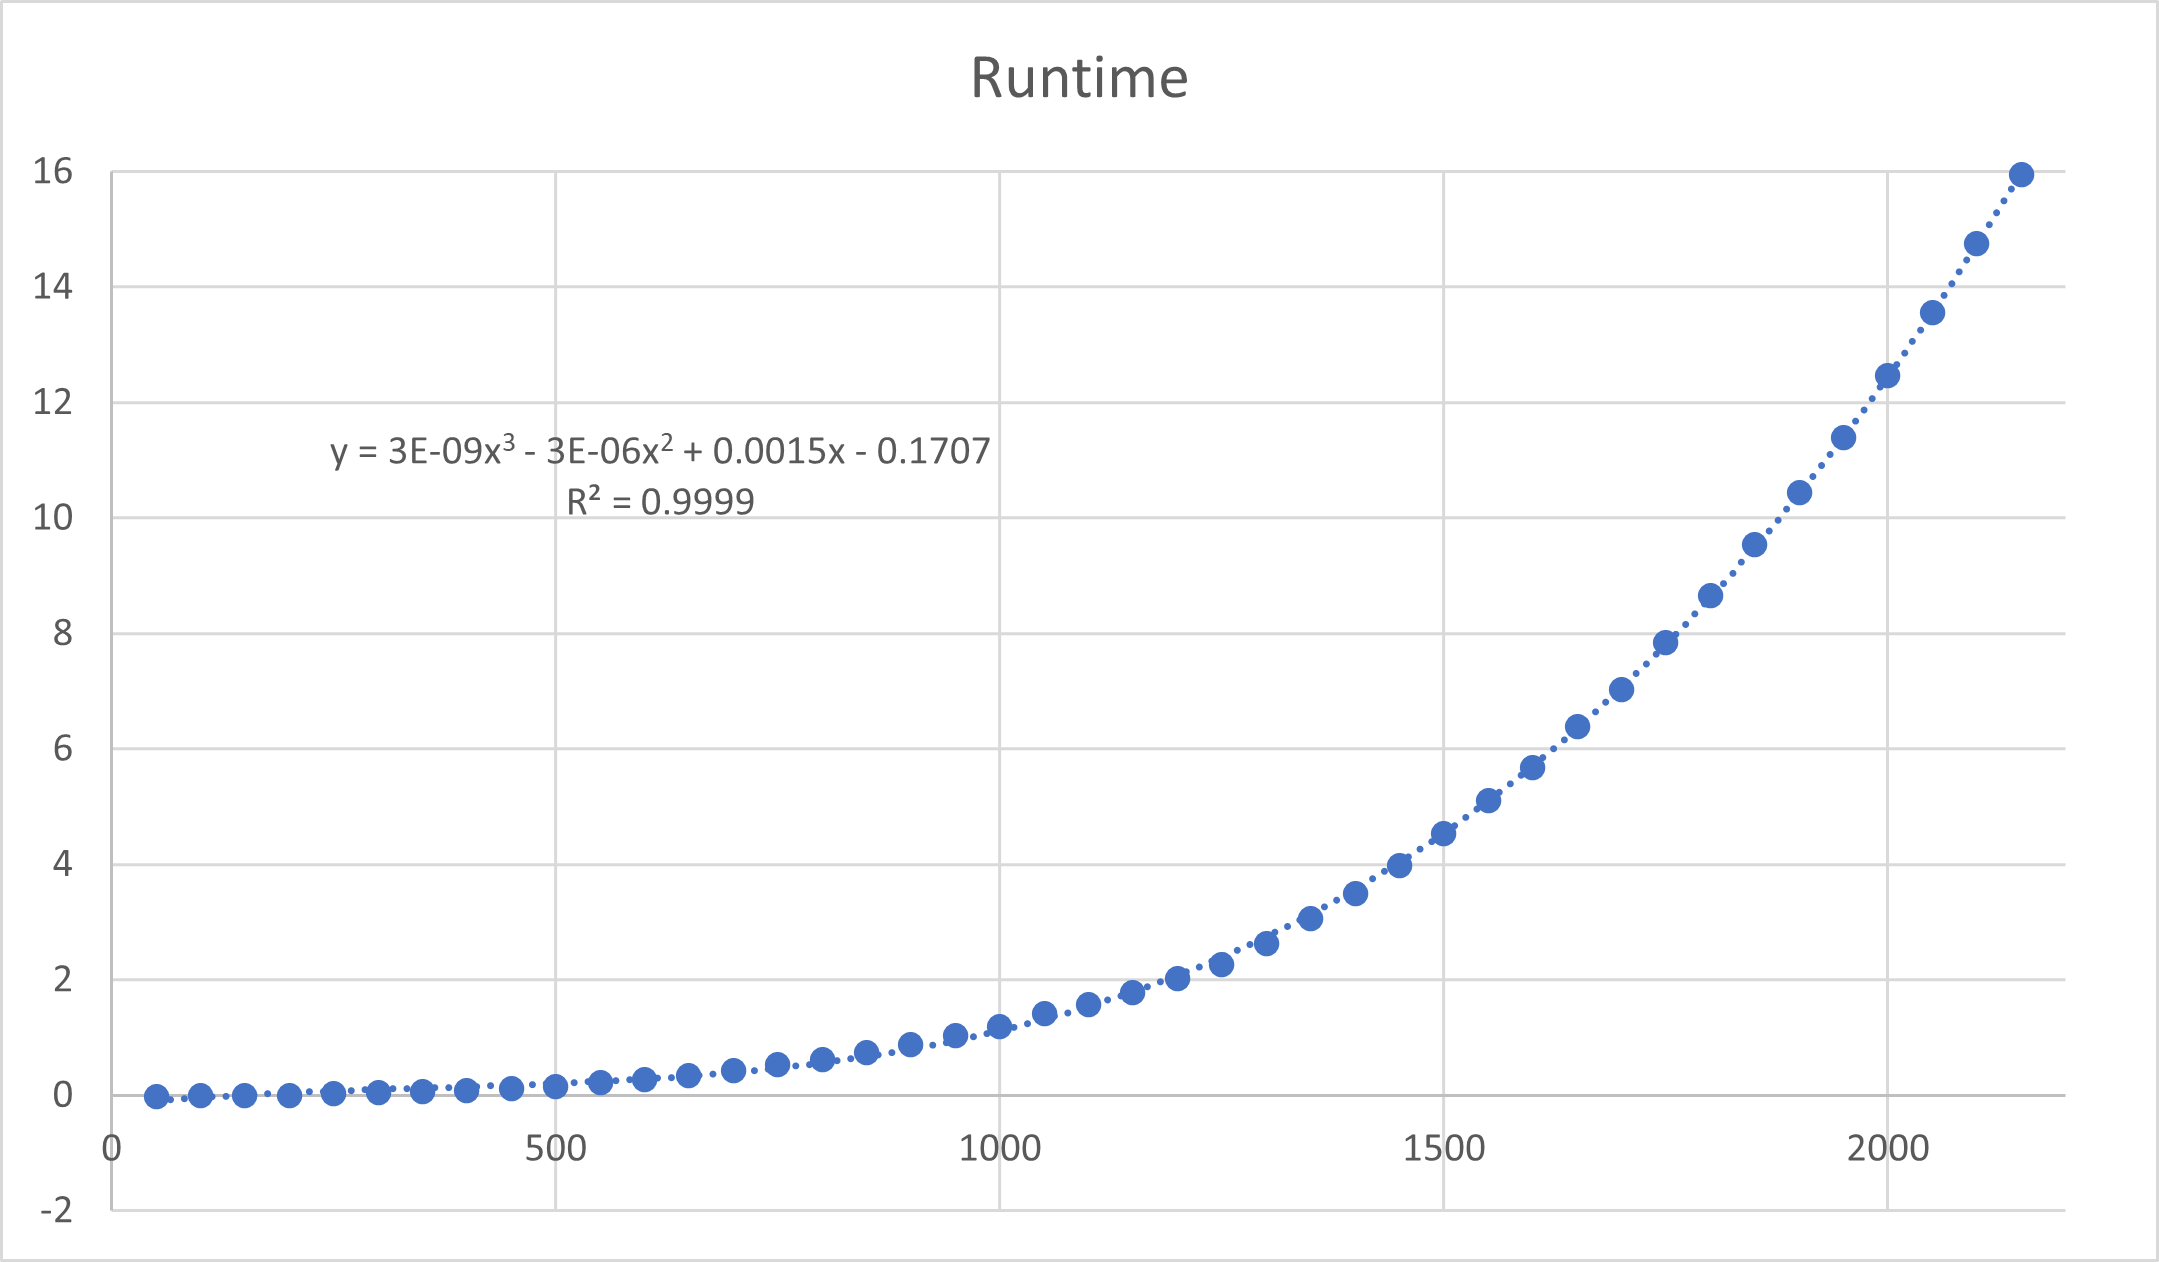
\includegraphics[width=0.6\textwidth,height=\textheight,keepaspectratio]{gn_Tn2}
\caption{linear fitting for $g(n)$}
\label{Figure: gn_3}
\end{figure}

\noindent Here, the $R^2$ is 0.9999, which is a very good result. Therefore we can conclude that $g(n) = O(n^3)$.

\subsection{\(h(n)\)}
When we graph the data set for $h(n)$, the trend line appears to be linear. From the chart below we can see that the $R^2$ is 0.9976 for the linear equation. This is already pretty good, but we might be able to improve it.

\begin{figure}[H]
\centering
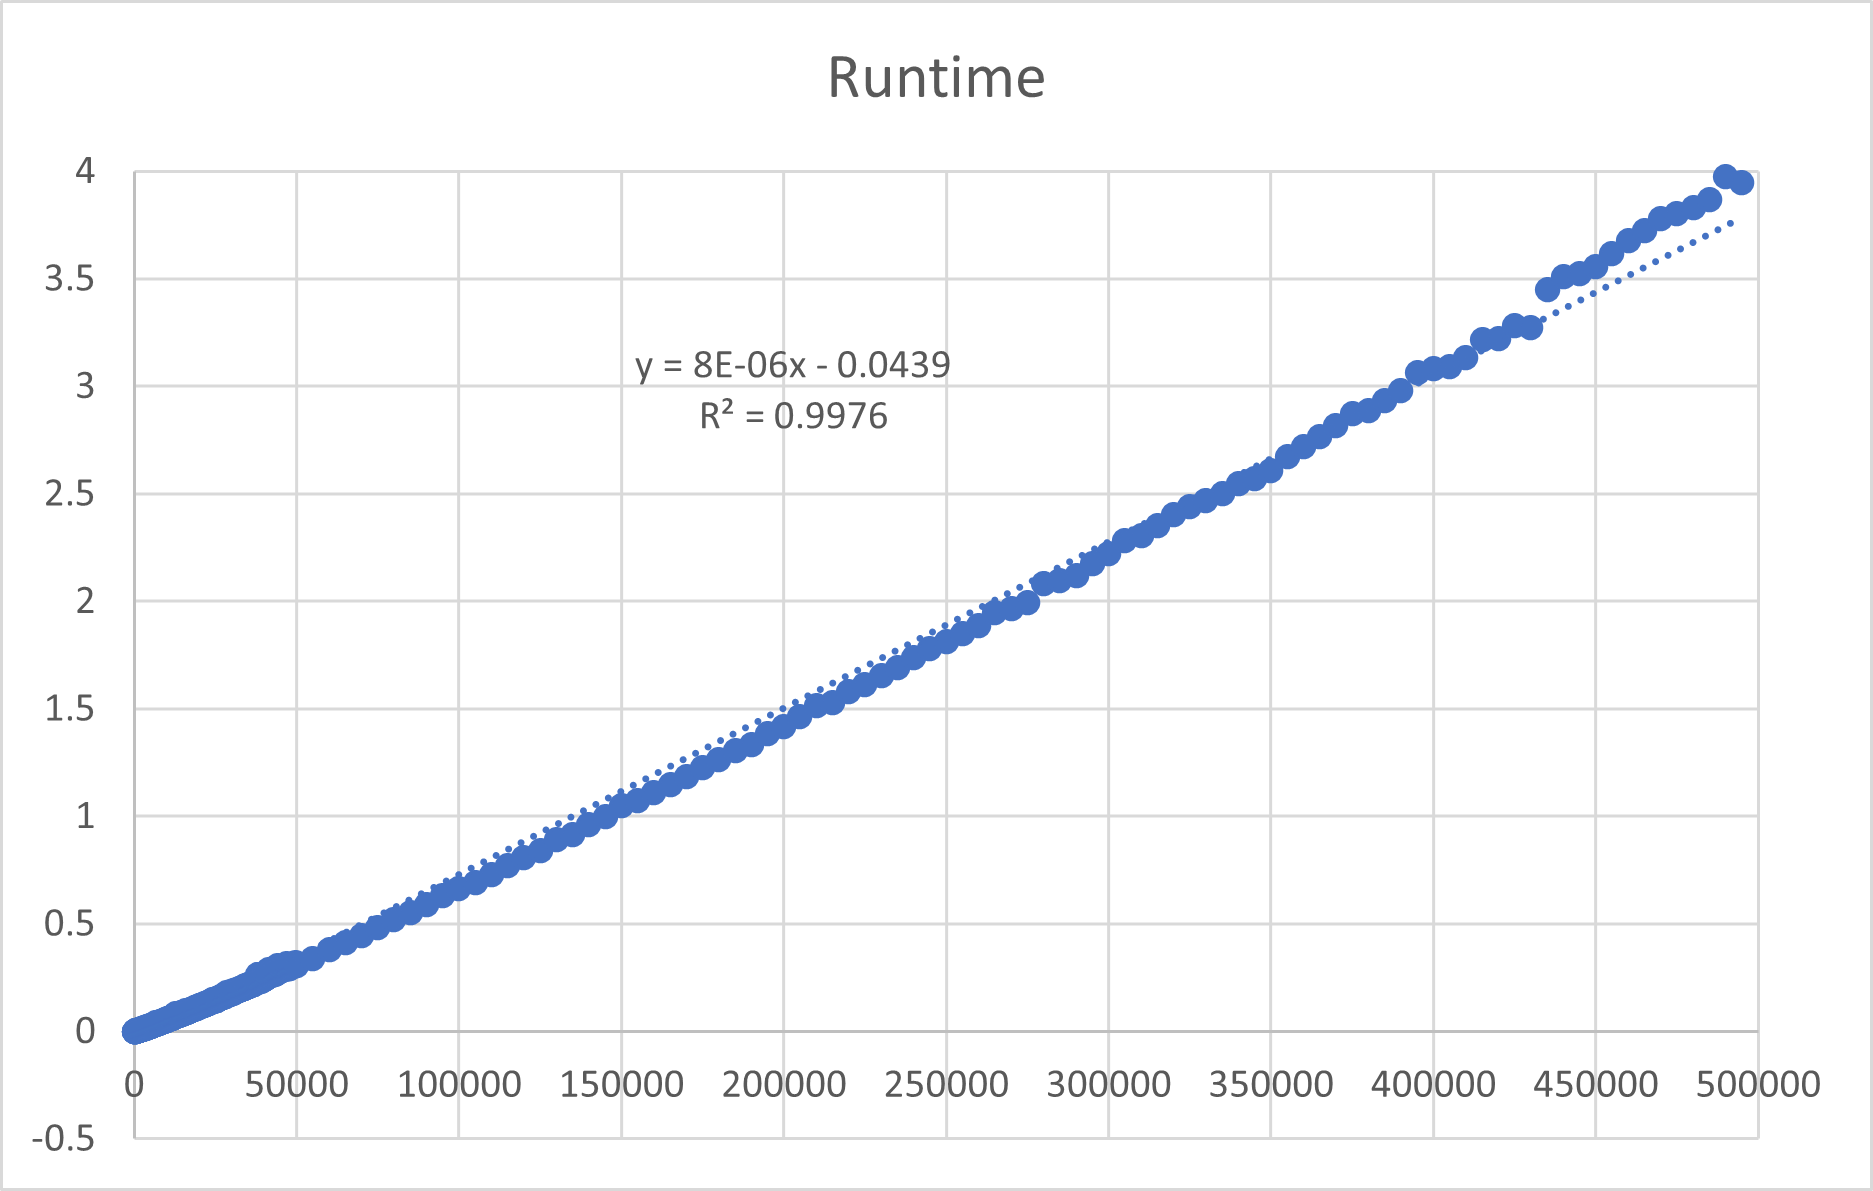
\includegraphics[width=0.6\textwidth,height=\textheight,keepaspectratio]{hn_Tn}
\caption{linear fitting for $h(n)$}
\label{Figure: hn_1}
\end{figure}

\noindent First, we will check the value of $k$ in $T(n) = cn^k$. We do so by taking the logarithm of both sides of this equation: $\log{T}=\log{c}+k\log{n}$ and plotting $\log{T}$ against $\log{n}$. 

\begin{figure}[H]
\centering
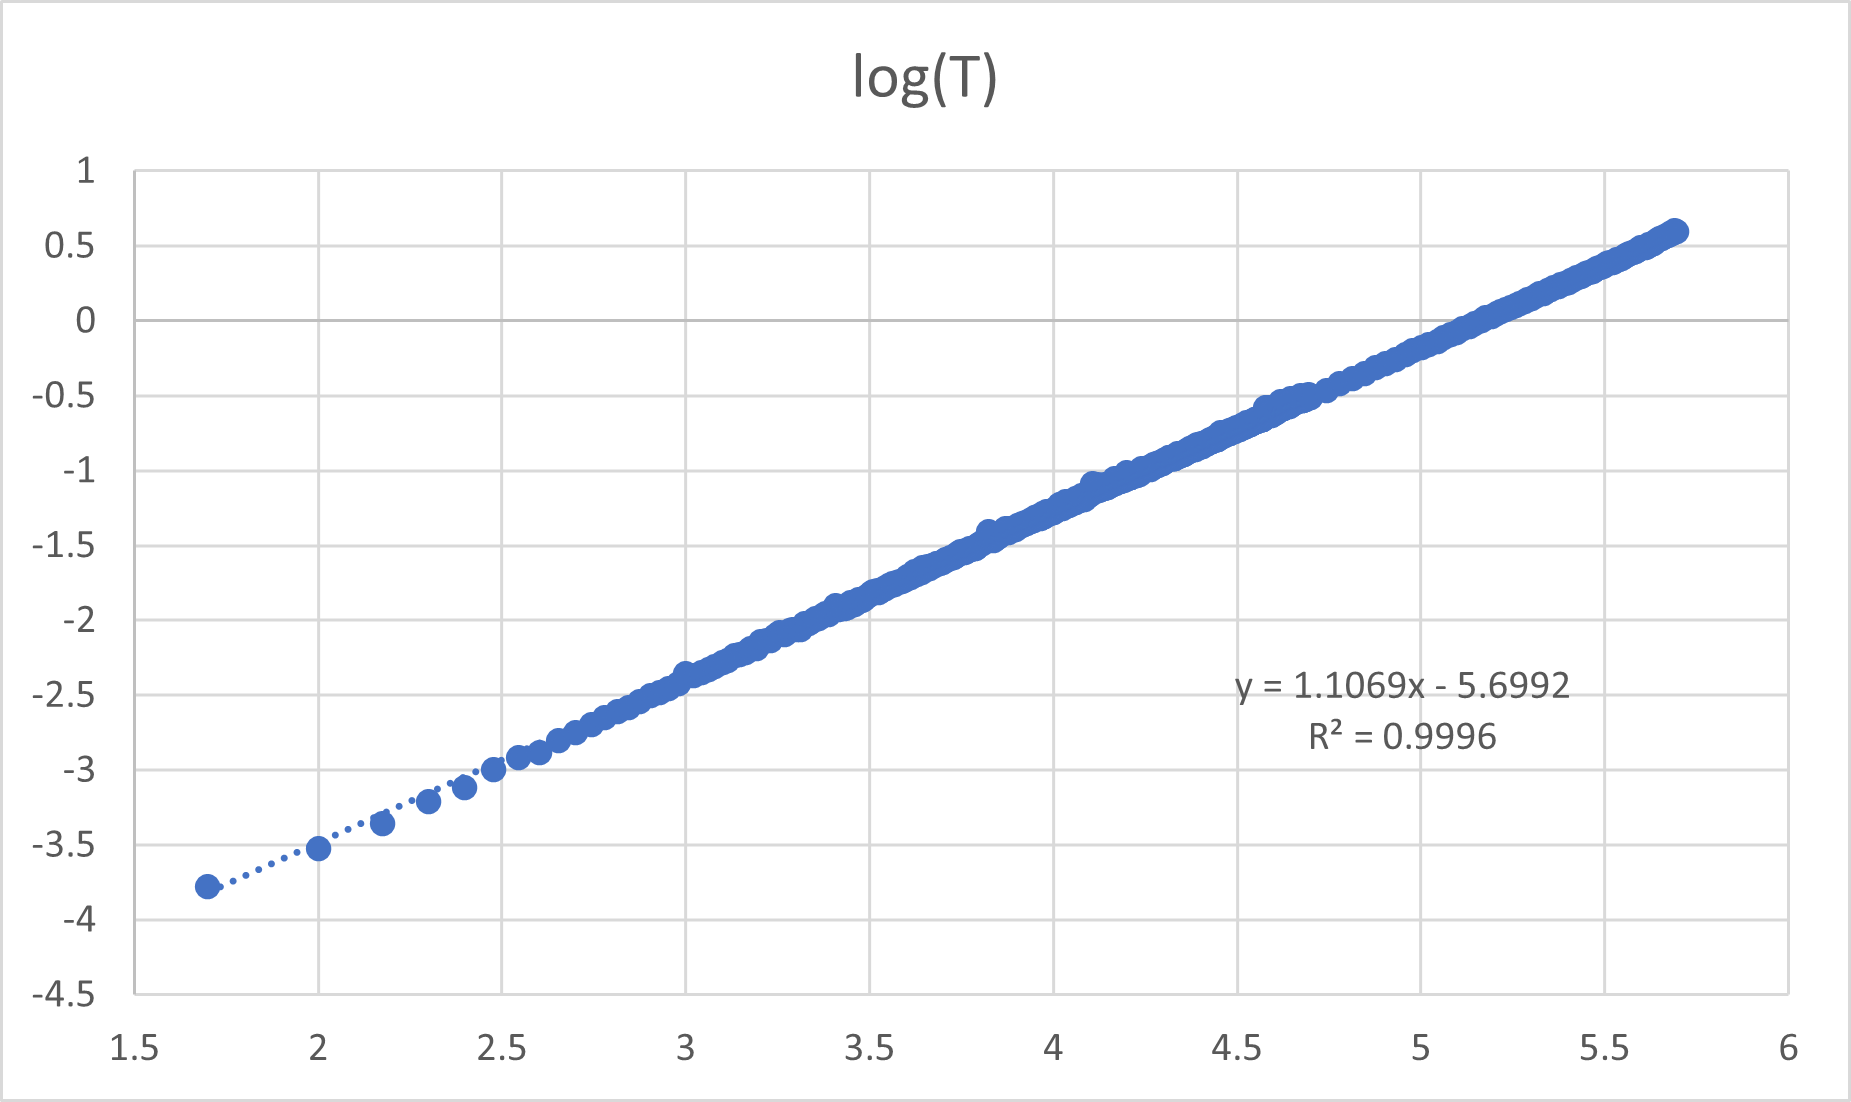
\includegraphics[width=0.6\textwidth,height=\textheight,keepaspectratio]{hn_logT}
\caption{linear fitting for $\log{T}$}
\label{Figure: hn_2}
\end{figure}

\noindent When we choose a linear trend line for this relation, we see that $k$, the slope, is 1.1069. Since $k$ represents the exponent on $n$ in the original data set, this makes the time complexity almost linear. However, $O(n\log{n})$ may be a better fit than $O(n)$. We can check which is better by plotting $\frac{T(n)}{n}$ against $n$. If $T(n) = cn$, then the resulting graph $\frac{T(n)}{n} = c$, will be linear. If $T(n) = cn\log{n}$, then the resulting graph $\frac{T(n)}{n} = c\log{n}$, will be logarithmic.

\begin{figure}[H]
\centering
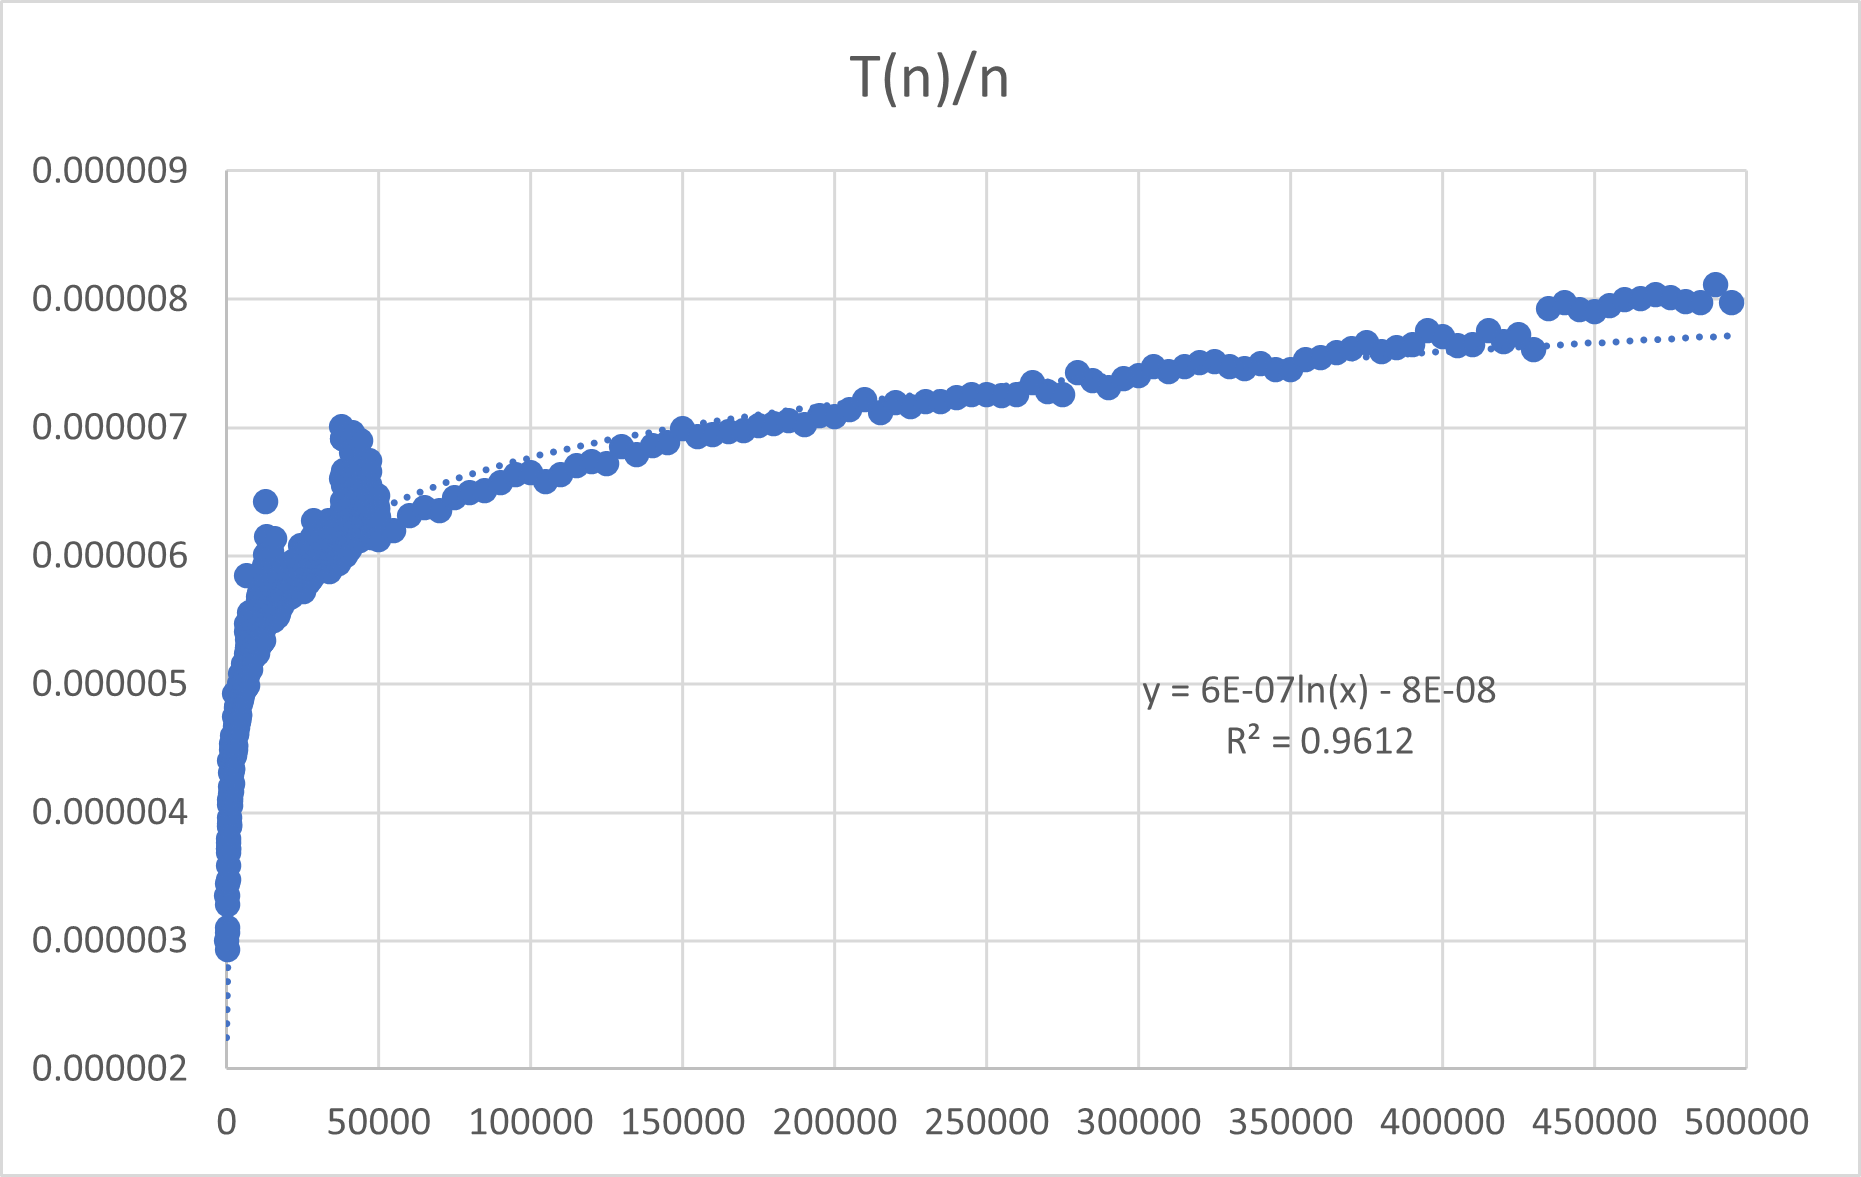
\includegraphics[width=0.6\textwidth,height=\textheight,keepaspectratio]{hn_Tn_n}
\caption{logarithmic fitting for $h(n)$}
\label{Figure: hn_3}
\end{figure}

\noindent The resulting graph appears to be logarithmic. The $R^2$ is 0.9612 for the logarithmic trend line. Therefore we can conclude that $h(n) = O(n\log{n})$.

\section{Python Lists}

\subsection{Copy}

\subsection{Lookups}

\subsection{Append}

\end{document}

